\section{Method}
\label{sec:method}
	
Short introduction on method 

%\noindent
\textit{FLORIS}: The FLOw Redirection and Induction in Steady state (FLORIS) model gives a two-dimensional approximation of the steady-state effect of yaw misalignment and axial induction. It creates a wake model with equation (\ref{eq:Dw} to \ref{eq:Uw}). 
\begin{figure}
  	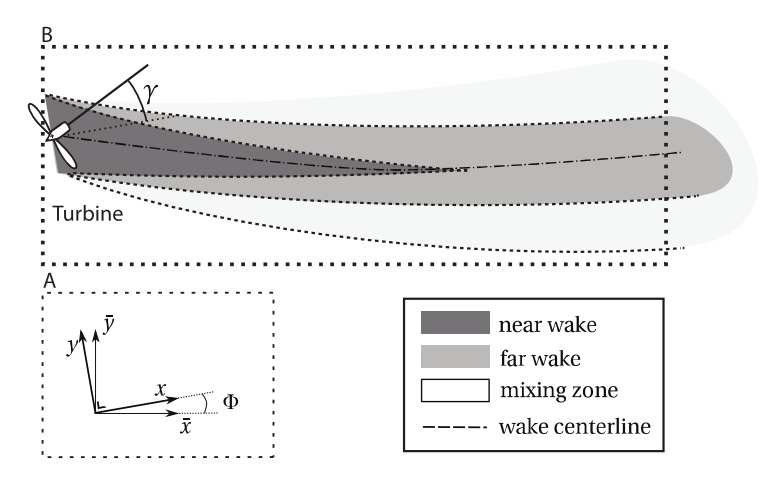
\includegraphics[width=\linewidth]{./Figures/WakeFLORIS.png}
  	\caption{Simplified repesentation of a wake by FLORIS.}
	\label{fig:wake}
\end{figure}
The wake is divided into three zones, $q_1$ to $q_3$, where $q_1$ refers to the near wake, $q_2$ to the far wake, and $q_3$ to the mixing zone (see Figure\ref{fig:wake}).
The size of the wake diameter $D_{w,q,i}$ increases proportionally to the the downwind distance ($x$). Let $D_i$ denote the diameter of the $i$th turbine, $k_e$ a coefficient that describes expansion of the zones \cite{Gebraad2016}, $m_{e,q}$ expansion factor. The diameter of the wake diameter is computed by,
\begin{equation}
\label{eq:Dw}
D_{w,i,q}(x) = max\left( {D_i + 2k_em_{e,q}([x - X_i],0} \right)
\end{equation}
The value $m_{U,q}$ is calculated with model parameters $a_U$, $b_u$, $M_{U,q}$, and computed as,
\begin{equation}
\label{eq:mU}
m_{U,q}(\gamma_i) =  \frac{M_{U,q}}{cos(a_U+b_U\gamma_i)}
\end{equation}
The value $c_{i,q}$ is the wake decay coefficient, which is calculated with,
\begin{equation}
\label{eq:c}
c_{i,q}(x) = \left[ \frac{D_i}{D_i + 2k_em_{U,q}(\gamma_i)[x - X_i]} \right]^2
\end{equation}
The axial induction factor is denoted by $a$ and the velocity deficit of the wake is calculated with,
\begin{equation}
\label{eq:Uw}
U_{w,i}(x,y) = U_i\left( {1-2a_ic_i(x,y)} \right)
\end{equation}
FLORIS gives a power output for each turbine, which for turbine $i$ is give by,
\begin{equation}
\label{eq:P}
P_i = \frac{1}{2} \rho A_i C_p(a_i, \gamma_i)U_i^3
\end{equation}
where, $\rho$ is the air density, $A$ the rotor area, U the wind velocity, and $C_p$ is equal to,
\begin{equation}
\label{eq:Cp}
C_p(a_i, \gamma_i) = 4a_i(1-a_i)^2 \eta cos(\gamma_i)^pP
\end{equation}
Where $\eta$ and $pP$ are power modeling parameters.
The values of the different parametric parameters are found in Table \ref{tab:para}
\begin{table}[h]
	%\renewcommand{\arraystretch}{1.3} 
	\caption{Overview of parametric parameters, with, the wake expansion factor for zone $i$ $m_{e,i}$, wake decay factor for zone $i$ $m_{U,i}$, wake decay parameters $a_U$ and $b_U$.}
	\centering
	\begin{tabular}{ll}
		\hline
		Expansion & Velocity  \\ 
		\hline
		$k_d \qquad \quad 0.15$ & $M_{U,1} \quad 0.5$ \\
		$m_{e,1} \quad -0.5$ & $M_{U,2} \quad 1$ \\
		$m_{e,2} \qquad 0.22$ & $M_{U,3} \quad 5.5$ \\
		$m_{e,3} \qquad 1$ & $a_U \qquad 5$ \\
		& $b_U \qquad 1.66$ \\
		\hline
		\label{tab:para}
	\end{tabular}
	
	Note: Table adjusted from Gebraad \cite{Gebraad2016}(nog correcte verwijzing toevoegen)
\end{table}

Although less accurate than  SOFWA high fidelity CFD simulation, computation time is much faster for FLORIS. As a result, FLORIS can be used for on-site optimization. 

%\noindent
\textit{FAST \& MLife}: FAST (Fatigue, Aerodynamics, Structures and Turbulence) is a programming tool for the simulation of dynamic (load) responses of wind turbines (by NREL) \cite{Jonkman2005}. It uses wind turbine specifications as well as wind flow situations. By evaluating a flow field, FAST computes the bending moment of a blade. MLife is an application to process the bending moment to compute the damage equivalent loads (DELs). 

\begin{figure}
  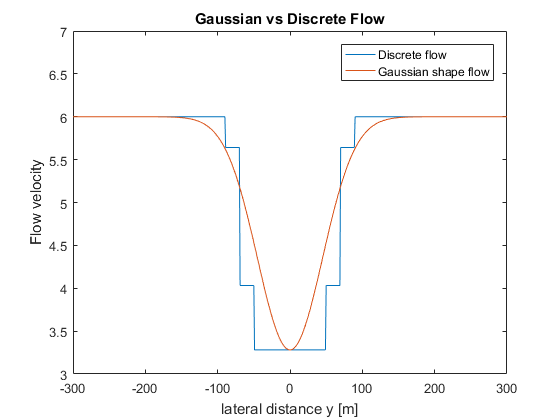
\includegraphics[width=\linewidth]{./Figures/PlotGausDiscWakeDWake180U6yaw0.png} %Plot with Gauss vs Discr flow, Dwake = 180, u_mean = 6, yaw = 0
  \caption{Discrete wake versus Gaussian wake} %for Dwake = 180 m, U = 6 m/s, and yaw = 0
  \label{fig:disgaus}
\end{figure}

%\noindent
\textit{Inflow files, Flow field}: FLORIS describes a discrete flow field of a wake, with three zones. The flow field of the wake in FLORIS is calculated with equations ((\ref{eq:Dw} to \ref{eq:Uw})). The wake is divided into three zones as described is in in the section on FLORIS. A real wake will not have discrete zones, but a more fluent transition between the wake zones (see Figure \ref{fig:disgaus} Plaatje van de gaussian vs discrete wake). To create a more fluent transition between the different wake-zones a Gaussian distribution of the flow field is preferred \cite{Bastankhah2016}. The Gaussian distribution is calculated as followed, 
\begin{equation}
\label{eq:gaus}
G(x, y) = A e^{-\frac{y^2}{2\sigma_y} + \frac{z^2}{2\sigma_z}}
\end{equation}
where the amplitude of the Gaussian, A, is equal to the velocity loss of the inner wake zone which is calculated with equation \ref{eq:Dw}. Values $\sigma_y$ and $\sigma_z$, in equation \ref{eq:gaus}, reflect the Gaussian standard deviation in horizontal and vertical direction, respectively. Both these standard deviations are linked to the spread of the Gaussian function. The standard deviations are linked to the outer wake zones, which are calculated by equations (numbers). In the model, $\sigma_y$ and $\sigma_z$ are a function of the diameter of the outer wake zone,  $D_{w,i,q=3}$, which is divided by a constant. This constant is equal to 4, which results in a standard deviation of two. As a result, the central 95.45\% of the values in the Gaussian distribution are taken. 

Wind shear can cause an important difference in velocity speeds between the rotor hub height, the end of the rotor blades at their highest points and the end of the rotor blades at their lowest point \cite{Firtin2011} (see Figure \ref{fig:windshear}). This velocity distribution is calculated with, 
\begin{equation}
\label{eq:shear}
v = v_{ref} \left[\frac{h}{h_{ref}}\right]^\alpha
\end{equation}
where $v$ and $v_{ref}$ are the velocity at heights $h$, and $h_{ref}$  respectively. Value $\alpha$ is the wind shear coefficient which depends on different factors. Coefficient $\alpha$ is fixed at value 0.1, reflecting a terrain type close to ocean and smooth ground \cite{Firtin2011}. The wind shear is implemented in the flow field.

\begin{figure}
\centering
   \begin{subfigure}[b]{0.50\textwidth}
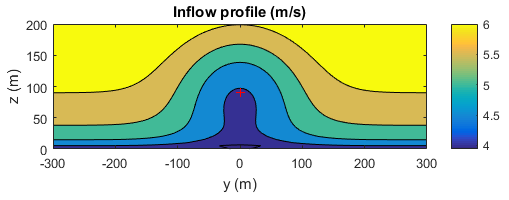
\includegraphics[width=\linewidth]{./Figures/PlotWindshearU6.png} %Plot with windshear u_mean = 6
  \caption{}
  \label{fig:windsh}
  \end{subfigure}

\begin{subfigure}[b]{0.50\textwidth}
    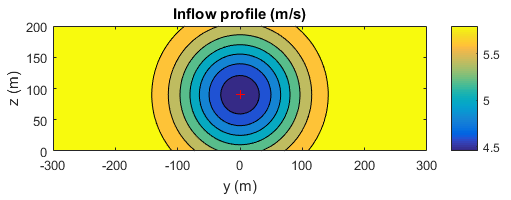
\includegraphics[width=\linewidth]{./Figures/PlotWithoutWindshearU6.png} %Plot without windshear u_mean = 6
  \caption{}
  \label{fig:nowindsh}
\end{subfigure}

\caption[Two Gaussian flow fields]{(a) Gaussian flow field with windshear. \\(b) Gaussian flow field without windshear.}
\label{fig:windshear}
\end{figure}



\begin{table}[h]
	%\renewcommand{\arraystretch}{1.3} 
	\caption{Overview of the minimum value, maximum value, and step size of the parameters, diameter of outer wake zone (Dwake), freestream wind speed (U), yaw of the turbine (yaw), and the center to center distance between the center of the turbine and the center of the wake (y wake).}
	\centering
	\label{tab:pars}
	\begin{tabular}{lccc}
		\hline
	 	& Minimum & Maximum & Step-size \\ 
		\hline
		Dwake & 180 & 330 & 25 \\
		U & 6 & 8 & 2 \\
		yaw & -30 & 30 & vary \\
		y wake & -250 & 250 & 10 \\
		\hline
	\end{tabular}
Note: Input values for yaw are [-30, -10, -5, 0, 5, 10, 30].
\end{table}

%\noindent
\textit{LUT}: To reduce computational time during optimization a look-up table (LUT) is created. The LUT is created using FAST and MLife, and it encompasses a wide variety of wind field conditions. 
These different conditions are described by the ranges of the parameters (see Table \ref{tab:pars}). The parameters are wake characteristics and can be extracted from FLORIS. The parameters chosen for the LUT are diameter of outer wake zone (Dwake), freestream wind speed (U), yaw of the turbine (yaw), and the center to center distance between the center of the turbine and the center of the wake (y wake). The output of the LUT are the DELs. The LUT generation is time consuming, as such, it cannot account for all integer values of the parameters. The step-size of these parameters is chosen such that interpolation will give a representative result. For each parameters step-sizes are selected, as shown in Table (see Table \ref{tab:pars}). With the use of the pre-calculated LUT, the optimization can run more swiftly, and is able to be used on-site.

\textit{verandwoording van de parameters}:

The ranges and stepsizes chosen for the individual parameters are selected so the LUT contains all the neseccery data needed to be able to generate an complete and accurate (beeld/afschatting) of every posible flowprofile.

this paper only looks at a 9 turbine case, for this case has a U range of 8to6m/s proven to be sufficient, lineair inperlopation is used to find values within these extremes. larger windfarms and different inflow wind velocities would require broadening these ranges.

de Dwake is op zo'n mannier gekozen dat ,bij normale omstandigheden, alle turbines binnen ... en ... meter kunnen worden gefit, de DEL relatie met de Dwake loopt mim of meer lineair, vandaar kon een relatief grote stepsize worden gekozen.

The yaw parameter is chosen at a stepsize of 10 degree, howerever extra data points were added at+-5 degree to improve the accuracy in the lower yaw regeones. the effect of this is shown in fig... 

the y wake parameter however fluctuates over its range, and could not be accurately estimated using lineair interpolation over large stepsizes. as mentioned in... .A stepsize of 10 meters, totaling a total of 51 steps, was found to be sufficiently accurate. 

 
 

%\noindent
\textit{Optimization}: Game Theory
\begin{figure}
  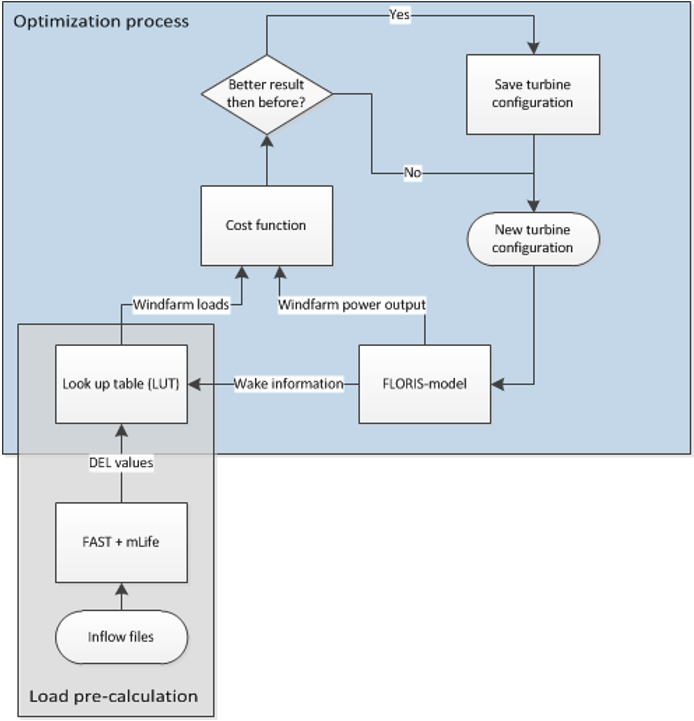
\includegraphics[width=\linewidth]{./Figures/OptimizationProcess.png}
  \caption{Overview of the optimalization procedure.}
  \label{fig:optim}
\end{figure}

